%%%%%%%%%%%%%%%%%%%%%%%%%%%%%%%%%%%%%%%%%%%%%%%%%%%%%%%%%%%%%%%%%%%%%%
% LaTeX Example: Project Report
%
% Source: http://www.howtotex.com
%
% Feel free to distribute this example, but please keep the referral
% to howtotex.com
% Date: March 2011 
% 
%%%%%%%%%%%%%%%%%%%%%%%%%%%%%%%%%%%%%%%%%%%%%%%%%%%%%%%%%%%%%%%%%%%%%%
% How to use writeLaTeX: 
%
% You edit the source code here on the left, and the preview on the
% right shows you the result within a few seconds.
%
% Bookmark this page and share the URL with your co-authors. They can
% edit at the same time!
%
% You can upload figures, bibliographies, custom classes and
% styles using the files menu.
%
% If you're new to LaTeX, the wikibook is a great place to start:
% http://en.wikibooks.org/wiki/LaTeX
%
%%%%%%%%%%%%%%%%%%%%%%%%%%%%%%%%%%%%%%%%%%%%%%%%%%%%%%%%%%%%%%%%%%%%%%
% Edit the title below to update the display in My Documents
%\title{Project Report}
%
%%% Preamble
\documentclass[paper=a4, fontsize=11pt]{scrartcl}
\usepackage[T1]{fontenc}
\usepackage{fourier}
\usepackage {listings}

\usepackage[english]{babel}															% English language/hyphenation
\usepackage[protrusion=true,expansion=true]{microtype}	
\usepackage{amsmath,amsfonts,amsthm} % Math packages
\usepackage[pdftex]{graphicx}	
\usepackage{url}


%%% Custom sectioning
\usepackage{sectsty}
\allsectionsfont{\centering \normalfont\scshape}


%%% Custom headers/footers (fancyhdr package)
\usepackage{fancyhdr}
\pagestyle{fancyplain}
\fancyhead{}											% No page header
\fancyfoot[L]{}											% Empty 
\fancyfoot[C]{}											% Empty
\fancyfoot[R]{\thepage}									% Pagenumbering
\renewcommand{\headrulewidth}{0pt}			% Remove header underlines
\renewcommand{\footrulewidth}{0pt}				% Remove footer underlines
\setlength{\headheight}{13.6pt}


%%% Equation and float numbering
\numberwithin{equation}{section}		% Equationnumbering: section.eq#
\numberwithin{figure}{section}			% Figurenumbering: section.fig#
\numberwithin{table}{section}				% Tablenumbering: section.tab#


%%% Maketitle metadata
\newcommand{\horrule}[1]{\rule{\linewidth}{#1}} 	% Horizontal rule

\title{
		%\vspace{-1in} 	
		\usefont{OT1}{bch}{b}{n}
		\normalfont \normalsize \textsc{} \\ [25pt]
		\horrule{0.5pt} \\[0.4cm]
		\huge Project 2 report \\
		\horrule{2pt} \\[0.5cm]
}
\author{
		\normalfont 								\normalsize
        Samy Shehata 22-3798\\[-3pt]		\normalsize
        Omar Mahmoud 22-1534\\[-3pt]		\normalsize
        Karim Tarek 22-0466\\[-3pt]		\normalsize
        \today
}
\date{}


%%% Begin document
\begin{document}
\maketitle
\section{Unification}
\subsection{Overview}
Unification is the process of determining if two first order logic expressions
are equivalent. This entails finding a most general unifier that enforces the
least number of bindings for variables to constants necessary to make the two
expressions equivalent. By applying a substitution of variables with constants
according to the MGU, we reach a common instance of the two expressions.

\subsection{Representation}
For unification, FOL expressions should be represented using lists. A list
represents a function or a predicate. First element of the list is the function
symbol, followed by its arguments. Arguments can either be lists (functions) or
atoms. Atoms are either variables or constants, both represented with their own
data types. A variable or a constant is defined as a \textit{struct} with field
\textit{sym}. \\
Ex:
\[
  P(a, y, f(y)) ->
  (list\ (make-predicate)\ \#\setminus P\ \#\setminus y\ (list\
  (make-predicate)\ \#\setminus f\
  \#\setminus y))
\]

\subsection{Implementation}

\subparagraph{Function Unify} \mbox{} \\
\noindent\textbf{Input}
\begin{itemize}
  \item {E1:} first expression listified
  \item {E2:} second expression listified
  \item {visual:} boolean
\end{itemize}
\noindent\textbf{Output}
\begin{itemize}
    \item{mu:} A list of bindings ( term / variable )
\end{itemize}
Tries to unify $E1$ and  $E2$ and returns the MGU if successful. Returns FAIL on
failure. If $viusal$ is true, the solution is traced step by step.

\subparagraph{Function unify1}
\begin{itemize}
  \item {E1:} first expression listified
  \item {E2:} second expression listified
  \item {mu:} A list of bindings {term / variable}
  \item {visual:} boolean
\end{itemize}
\noindent\textbf{Output}
\begin{itemize}
    \item{mu:} A list of bindings ( term / variable )
\end{itemize}
Recursive helper function to Unify, carries out the bulk of unification. Takes the two
expressions and mu which is the MGU so far. Unifies the first two elements in
$E1$ and $E2$, updates the MGU and then continues on the rests of the two expressions.
This function follows the algorithm described in class.

\subparagraph{Function unify-var}
\begin{itemize}
  \item {x:} an FOL variable
  \item {e:} an FOL term to be unified with x
  \item {mu:} A list of bindings {term / variable}
  \item {visual:} boolean
\end{itemize}
\noindent\textbf{Output}
\begin{itemize}
    \item{mu:} A list of bindings ( term / variable )
\end{itemize}
Helper function to $unify1$, called when a variable is encountered in one of the
expressions. Takes the variable x, the corresponding term $e$ from the other
expression and mu (the MGU so far). If $x$ is not bound according to mu the $x$
is bound to $e$ and mu is updated, otherwise $e$ is unified with the binding of $x$.
unify-var fails if $x$ needs to be bound to a term that also contains $x$.

Smaller helper functions are documented in the code.

\subsection{Sample Runs}
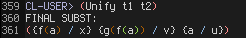
\includegraphics[width=0.5\textwidth]{unfiy.png}
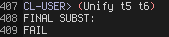
\includegraphics[width=0.5\textwidth, height=1.1cm]{unify-fail.png}
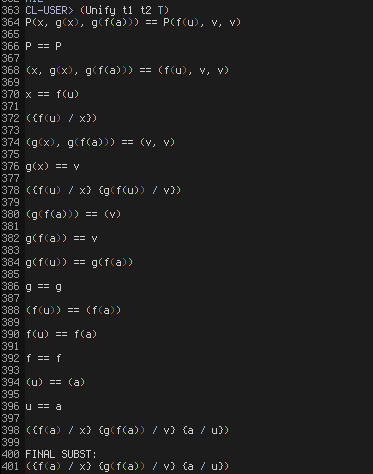
\includegraphics[width=0.5\textwidth]{trace-unify.png}

\subsection{How To Run}
Loading the runme.lisp file will compile the code and show a test run with the
examples from the project description (please ignore compilation style warnings).
To load the file in Top-level lisp REPL: \\
\begin{lstlisting}
(load ``runme.lisp'')
\end{lstlisting}
At this point, the example inputs are defined in variables $t1$ - $t6$ and can be
used as:
\begin{lstlisting}
(Unify t1 t2)
\end{lstlisting}
for normal mode and 
\begin{lstlisting}
(Unify t1 t2 T)
\end{lstlisting}
for trace mode. In trace mode, you can press (Enter key) to advance to the next
step.

\section{Clause Form}
\subsection{Overview}
Clause form is a representation of first order logic
statements as a conjunction of clauses, where each clause is a disjunction of
literals.


\subsection{Representation}
For ClauseForm, FOL expressions are represented as lists, where the first
element of the list is an operator and the rest of the list are the operands.
Each operator is represented as with their own data type using structs. The
defined operators are (land, lor, limpl, leq, forall, there-exists and lnot) for
(logical and, or, implication, equivelance, for all, there exists and not).
Literals are also represented as a list with struct $latom$ as the first
element. The struct holds the function symbol and the literal arguments form the
rest of the list. 
Ex: \\
\[
  \forall x[P(x)] = \\
  (list\ (make-forall\ :sym\ x)\ (list\ (make-latom\ :sym\ P)\
  x)) 
\]

\subsection{Implementation}


\subparagraph{Function ClauseFrom}
\begin{itemize}
  \item {expr:} FOL expression listified
  \item{visual:} boolean
\end{itemize}
\noindent\textbf{Output}
\begin{itemize}
    \item{expr:} FOL expression listified
\end{itemize}
Takes FOL expression and applies the clause form steps then returns the clause
form expression. If visual is true, the solution is traced step by step.

\subparagraph{Function remove-eql}
\begin{itemize}
  \item {expr:} FOL expression listified
\end{itemize}
\noindent\textbf{Output}
\begin{itemize}
    \item{expr:} FOL expression listified
\end{itemize}
Recursively looks for expressions of the form $ (list\ leq\ a\ b) $ and changes
them to $(list\ land\ (list\ limpl\ a\ b)\ (list\ limpl\ b\ a))$


\subparagraph{Function remove-impl}
\begin{itemize}
  \item {expr:} FOL expression listified
\end{itemize}
\noindent\textbf{Output}
\begin{itemize}
    \item{expr:} FOL expression listified
\end{itemize}
Recursively looks for expressions of the form $ (list\ limpl\ a\ b) $ and changes
them to $(list\ lor\ (list\ not\ a)\ b)$


\subparagraph{Function push-not}
\begin{itemize}
  \item {expr:} FOL expression listified
\end{itemize}
\noindent\textbf{Output}
\begin{itemize}
    \item{expr:} FOL expression listified
\end{itemize}
Recursively looks for expressions of the form $ (list\ not\ a) $ and applies the
not operation on $a$ recursively until a literal is hit. The not operations
changes $\forall$ to $\exists$ and the reverse, $(list\ land\ a\ b)$ to $(list\ lor\ (list\
lnot\ a) (list\ lnot\ b)$. The reverse is done to ors.


\subparagraph{Function standarise-apart}
\begin{itemize}
  \item {expr:} FOL expression listified
\end{itemize}
\noindent\textbf{Output}
\begin{itemize}
    \item{expr:} FOL expression listified
\end{itemize}
Recursively looks for expressions with quantifiers, the symbol of the
quantifiers is added to a list of used variables. If found again in another
quantifier, all variables within the scope of the quantifier are renamed.

\subparagraph{Function skolemize-apart}
\begin{itemize}
  \item {expr:} FOL expression listified
\end{itemize}
\noindent\textbf{Output}
\begin{itemize}
    \item{expr:} FOL expression listified
\end{itemize}
Recursively looks for expressions with $\exists$,  the variable  within the
scope of the quantifier are renamed to skolem variables.


\subparagraph{Function discarded-apart}
\begin{itemize}
  \item {expr:} FOL expression listified
\end{itemize}
\noindent\textbf{Output}
\begin{itemize}
    \item{expr:} FOL expression listified
\end{itemize}
Recursively looks for expressions of the form $(list\ (forall) a)$, and changes
them to $a$.

\subparagraph{Function flatten-apart}
\begin{itemize}
  \item {expr:} FOL expression listified
\end{itemize}
\noindent\textbf{Output}
\begin{itemize}
    \item{expr:} FOL expression listified
\end{itemize}
Recursively changes all nested expressions to a top $and$ expression, with all
operands being $or$ expressions of literals.

\subparagraph{Function flatten-apart}
\begin{itemize}
  \item {expr:} FOL expression listified
\end{itemize}
\noindent\textbf{Output}
\begin{itemize}
    \item{expr:} FOL expression listified
\end{itemize}
Recursively changes all nested expressions to a top $and$ expression, with all
operands being $or$ expressions of literals.


\subparagraph{Function clauses}
\begin{itemize}
  \item {expr:} FOL expression listified
\end{itemize}
\noindent\textbf{Output}
\begin{itemize}
    \item{expr:} FOL expression listified
\end{itemize}
Takes a cnf expression and returns a list of lists where the inner lists are the
disjunctions and the outer list is the conjunction,

\begin{itemize}
  \item {expr:} FOL expression listified
\end{itemize}
\noindent\textbf{Output}
\begin{itemize}
    \item{expr:} FOL expression listified
\end{itemize}
Takes a list of lists and renames the variables within them such that no
variable is shared among two lists.

Smaller helper functions are documented in code.


\subsection{Sample Runs}
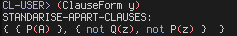
\includegraphics[width=0.5\textwidth]{cnf.png} \\
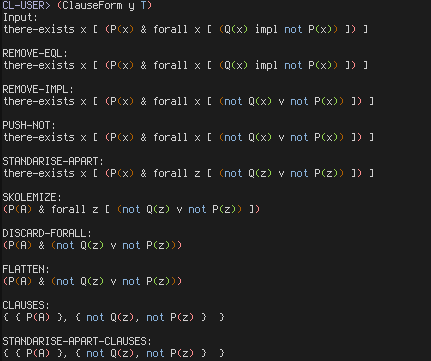
\includegraphics[width=0.5\textwidth, height=8cm]{cnf-trace.png} \\

\subsection{How To Run}
Loading runme.lisp also compiles the code for clause form and creates two
variables $ y$ and $z$ for example inputs from the project description.
\begin{lstlisting}
(load ``runme.lisp'')
\end{lstlisting}
Then clause form can be called as
\begin{lstlisting}
(ClauseFrom y)
\end{lstlisting}
for normal mode, and
\begin{lstlisting}
(ClauseForm y T)
\end{lstlisting}
for trace mode. In trace mode you can press (Enter key) to advance to the next
step in the solution.
%%% End document
\end{document}
